\documentclass[twoside, a4paper, twocolumn]{article}
\usepackage[english]{babel}
\usepackage{a4wide}

% Fonts
\usepackage[sc]{mathpazo}
\usepackage[T1]{fontenc}
\linespread{1.05}
\usepackage{microtype}
\usepackage{lettrine}

% References
\usepackage{varioref}
\usepackage{hyperref}
\usepackage{cleveref}

% Document layout
% \usepackage[hmarginratio=1:1,top=32mm,columnsep=20pt]{geometry}
% \usepackage{multicol}
\usepackage{paralist}

% Floats
\usepackage{float}
\newenvironment{Figure}
  {\par\medskip\noindent\minipage{\linewidth}}
  {\endminipage\par\medskip}

%Plaatjes
\usepackage{graphicx}
\usepackage[small,labelfont=bf,up,textfont=it,up]{caption}
\usepackage{subcaption}

% Tables
\usepackage{booktabs}

% Custom section headers
\usepackage{titlesec}
\renewcommand\thesection{\Roman{section}}
\renewcommand\thesubsection{\Roman{subsection}}
\titleformat{\section}[block]{\large\scshape\centering}{\thesection.}{1em}{}
\titleformat{\subsection}[block]{\large}{\thesubsection.}{1em}{}

% Code
\usepackage{color}
\usepackage{listings}
\definecolor{Blue}{rgb}{0,0,0.5}
\definecolor{Green}{rgb}{0,0.75,0.0}
\definecolor{LightGray}{rgb}{0.6,0.6,0.6}
\definecolor{DarkGray}{rgb}{0.3,0.3,0.3}
\lstset{language=Matlab,
   keywords={function,uint8,uint16,uint32,double,break,case,catch,continue,else,elseif,end,for,global,if,otherwise,persistent,return,switch,try,while},
   basicstyle=\ttfamily\small,
   breaklines=true,
   keywordstyle=\bfseries\color{Blue},
   commentstyle=\itshape\color{LightGray},
   stringstyle=\color{Green},
   numbers=left,
   numberstyle=\tiny\color{DarkGray},
   stepnumber=4,
   numbersep=10pt,
   backgroundcolor=\color{white},
   tabsize=2,
   showspaces=false,
   showstringspaces=false,
   captionpos=b
}

%Wiskunde
\usepackage{siunitx}
\usepackage{mathtools}
\usepackage{amsmath}
\usepackage{amsfonts}
\usepackage{amssymb}

% References
\usepackage[backend=bibtex]{biblatex}
\usepackage{csquotes}
\bibliography{biblio}

% Pseudo code
\usepackage{setspace}
\usepackage[algoruled,vlined, linesnumbered, shortend]{algorithm2e}

% Temp
\usepackage{todonotes}

% Math commands
\newcommand{\normal}[2]{\ensuremath{\mathcal{N}\left(#1,\, #2\right)}}
% \renewcommand{\vec}[1]{\ensuremath{\mathbf{#1}}}

% Other commands
\renewcommand{\t}[1]{\texttt{#1}}

\DeclarePairedDelimiter\abs{\lvert}{\rvert}%
\DeclarePairedDelimiter\norm{\lVert}{\rVert}
\makeatletter
\let\oldabs\abs
\def\abs{\@ifstar{\oldabs}{\oldabs*}}
\let\oldnorm\norm
\def\norm{\@ifstar{\oldnorm}{\oldnorm*}}
\makeatother

\title{Neural Networks\\Practical Assignment 2: Learning a Rule}
\author{Rick van Veen (s1883933) \and Laura Baakman (s1869140)}

\begin{document}

\twocolumn[\maketitle]


% \todo[inline]{Use compactitem environment for lists}

% Example table:
% \begin{table}[H]
% \caption{Example table}
% \centering
% \begin{tabular}{llr}
% \toprule
% \multicolumn{2}{c}{Name} \\
% \cmidrule(r){1-2}
% First name & Last Name & Grade \\
% \midrule
% John & Doe & $7.5$ \\
% Richard & Miles & $2$ \\
% \bottomrule
% \end{tabular}
% \end{table}

% \begin{multicols}{2}

\section{Introduction}
%!TEX root = practicum3.tex
In this report we consider a multilayer feed forward neural network, which we will train using the stochastic gradient descent algorithm. Gradient descent (GD) is an optimization algorithm which tries to find the local minimum of a function, by taking steps proportional to the negative of the gradient at a certain point. In the case of a feed forward network gradient descent is applied to minimize the cost function (see \eqref{eq:1:cost} and \cref{s:method} for the explanation of this function) and thus by doing so hoping to find the solution with the lowest cost. 

The stochastic gradient descent (SGD) algorithm in contrast to the GD algorithm does not use the gradient of the cost function, but the gradient of the contribution (see \eqref{eq:1:contribution} and \cref{s:method} for the explanation) of a randomly sampled data point. The reason why SGD is used apposed to GD is whenever the (training) data set is very large, GD has to go through the whole training set in order to perform an update. SGD on the other hand only takes one data point and updates its weights immediately and thus also immediately starts to increase its performance \cite{bottou2010large}.

	
\section{Method}
\label{s:method}
%!TEX root = practicum1.tex
Given a dichotomy $\mathcal{D} = \left\{\xi^i, S^i \right\}_{i}^{N}$ with $N$ $d$-dimensional patterns $\xi \in \mathcal{R}^d$, each with a label $S \in \left\{-1, +1 \right\}$, a perceptron can be trained using the Rosenblatt algorithm \todo[inline]{Add a reference to the Rosenblatt algorithm} which updates the weights each time step $t = 1, 2, \ldots$:
	\begin{equation}\label{eq:1:rosenblat}
		\vec{w}(t+1) = 
		\begin{cases}
		\vec{w}(t) + \frac{1}{d} \xi^{\mu(t)} S^{\mu(t)}
		& \text{if } E^{\mu(t)} \leq 0\\
		\vec{w}(t) 											
		& \text{otherwise}\\
		\end{cases}
	\end{equation}
Where $\mu(t) = 1, 2, \ldots, N, 1, 2, \ldots$ is used to select the next pattern to train with. The energy function $E(\cdot)$, anagolous to the local action potential in a biological neuron, is defined as:
	\begin{equation}\label{eq:1:energyFunction}
		E^{\mu(t)} = \vec{w}(t) \cdot \xi^{\mu(t)}S^{\mu(t)}.
	\end{equation}
The energy function indicates if the perceptron gives the correct output for the given input pattern $\xi^{\mu(t)}$. Since we know that independent of the initial value of the weights the perceptron will converge, if the $\mathcal{D}$ is linearly separable, the initialization of the weights is irrelevant. We have opted for $\vec{w}(0) = 0$.\\

The update defined in \autoref{eq:1:rosenblat} is executed until $E^{\xi^i} > 0$ for $i \in [1, N]$, if this is the case the algorithm has converged. If the dataset is not linearly separable the perceptron never converges, thus it is generally a good idea to set a maximum number epochs, $d_{max}$, where each epoch consists of $N$ steps. The total number of steps taken by the algorithm has thus the upper bound $d_{max} \cdot N$. \\


\todo[inline]{Dit stukje naar de intro verplaatsen, bij het linearly separable stukje}
\textcite{cover1965geometrical} showed that the probability that a randomly chosen dichotomy  in general position is linearly separable can be proven to be:
	\begin{equation}\label{eq:1:lsChance}
		f(N,d) = 
		\begin{cases}
		1
		& N \leq d + 1\\
		\frac{2}{2^N} \displaystyle\sum_{k = 0}^{d} \binom{N - 1}{k}										
		& \text{otherwise}\\
		\end{cases}
	\end{equation}
To verify this theoretical result we have performed two experiments.


	

\section{Experiment}
%!TEX root = practicum2.tex
The performance of the perceptron trained with the Minover algorithm can be measured using the generalization error defined in \autoref{eq:method:generalization_error}. To explore the behaviour of the Minover algorithm discussed in section \ref{s:method} we have tested a perceptron trained with this algorithm on several $N$-dimensional datasets with $P = \alpha N$, for $N = 10$ and $\alpha = 0.1, 0.2, \dotsc, 5$. To ensure that the dataset was linearly separable we have determined its labels via \eqref{eq:method:teacher_label}, using the weight vector $\vec{w}^* = [1, \dotsc, 1]^T$.\\

\begin{figure}[b]
	\centering
	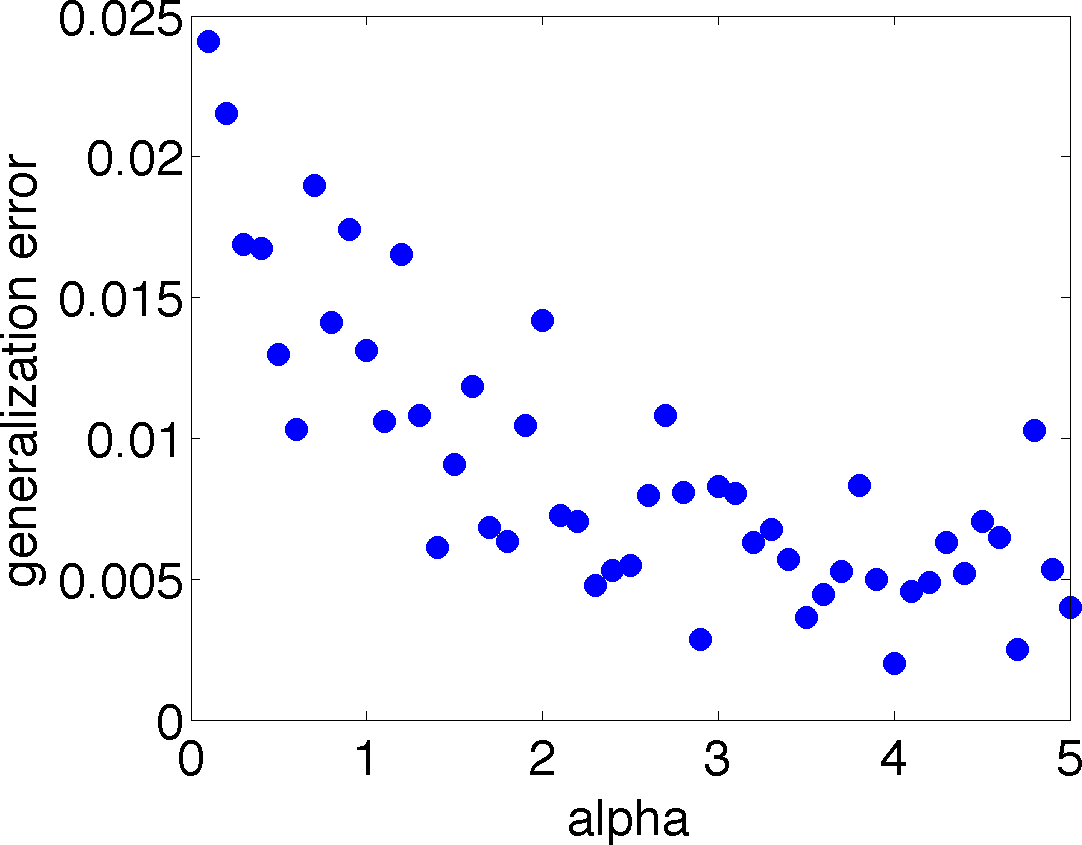
\includegraphics[width=0.9\columnwidth]{./img/finalgeneralizationerrors}
	\caption{Generalization error at the final step of training as an average of twenty iterations for $\alpha = 0.1, 0.2, \dotsc, 5$, $\varepsilon = 0.0005$, $n_{max} = 500$ and $N = 10$.}
	\label{fig:exp:finalgeneralizationError}
\end{figure}

\Cref{fig:exp:finalgeneralizationError} shows the generalization error, between the student and teacher perceptron, for different values of $\alpha$ as an average of $n_d = 20$ iterations with each $\alpha$. We consider a generalization error final when it has converged or when $t_{max}$ has been reached as explained in \cref{s:method}. 

Based on \cref{fig:exp:finalgeneralizationError} we can state that the generalization error decreases as $\alpha$ increases. A small $\alpha$ results in a smaller number of patterns, this means that it is more probable that the teacher is not the optimal solution. Because of this the generalization error is likely to be larger than with a large $\alpha$ which results in a larger number of patterns and less possible solutions, thus meaning a higher probability the teacher lies near (or is) the solution with maximum stability.

The fluctuations in the $\epsilon_g$ in \cref{fig:exp:finalgeneralizationError} may be due to the random data sets.\\
	

\printbibliography


\appendix
\twocolumn[
\section{Implementation}
\label{ap:matlab}

\lstinputlisting{../code/minover.m}
]
% \end{multicols}
\end{document}

